\chapter{Matchings}
    A \textbf{matching} of a graph $G$ is a set of non-loop edges such that no 2 edges share an end.\\
    $\emptyset$ is a matching
    \section{Matching in a bipartite graph}
        \begin{description}
            \item[$\nu(G)$]: max size (number of edge) of a matching of $G$\\
                \begin{figure}[h]
                    \centering
                    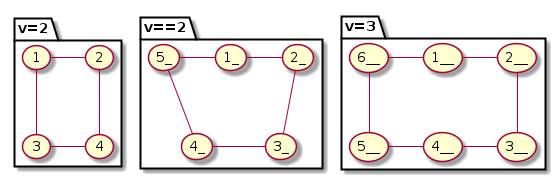
\includegraphics[scale=0.5]{ressources/images/NuG.png}
                    \caption{Examples of $\nu(G)$}
                    \label{Tree}
                \end{figure}
            \item[$\tau(G)$]: min number vertices that meet every edge\\
                ($min|x|:x\subseteq V(G)$ every edge has at least 1 end in $X$)
            \item[$M$-alternating path] is a path $P=v_0 e_1 v_1 e_2 v_2 e_3 v_3 e_4 \cdots e_n v_n$ such that $e_2, e_3, \cdots \in M$
            \item[$M$-augmenting path] is a path $P=v_0 e_1 v_1 e_2 v_2 e_3 v_3 e_4 \cdots e_n v_n$ such that $P$ is $M$-alternating and $V_0 V_n$ are not incident with any edge in $M$
        \end{description}
        \subsection{König's theorem}
            $G$ bipartite $\Rightarrow$ $\nu(G)=\tau(G)$
        \subsection{Proof}
        \subsection{Lemma}
            Let $M$ be a matching of a graph $G$\\
            $M$ is a maximum matching $\Leftrightarrow$ $G$ has no $M$-augmenting path
        \subsection{Proof}
            \begin{description}%TODO: finish
                \item[$\Rightarrow$] If $P$ is an $M$-augmenting path\\
                    Let $M'=M\Delta E(P)$ ($X\Delta Y=(X-Y)\cup(Y-X)$)\\
                \item[$\Leftarrow$]: \textbf{$\tau(G)\geq \nu(G)$}: Trivial (Even works for all graphs)\\
                \textbf{$\tau(G)\leq \nu(G)$}: Let $k=\nu(G)$\\
                        Let $M$ be a matching of size $k$.\\
                        \textbf{We want to find a set of $k$ vertices meeting every edges}
                        Let $(A, B)$ be a bipartition of $H$\\
                        \textit{$G$ has no $M$-augmenting path}

                        Let $A'=A-V(M)$\\
                        Let $B_0$ be the subset of $B$ that can be reached from $A'$ by an $M$-alternating path.\\
                        Let $A_0=$subset of $A$ incident with an edge in $M$\\
                        Let $A_1=A-A_0-A'$\\
                        \textbf{CLAIM}: Every edge is incident with a vertex in $A_1\cap B_0$ $\Rightarrow$ \textbf{TRUE}
            \end{description}
        \subsection{Hall's theorem}
            Let $G$ be a bipartite grpah with a bipartition $(A, B)$\\
            $G$ has a matching $M$ covering $A$ $\Leftrightarrow$ $\forall S \subseteq A, |N_{G}(S)|\geq|S|$ (With $N_{G}(S)$=set of all neighbours of $G$ vertices in $S$)\\
        \subsection{Proof}
            \begin{description}
                \item[$\Leftarrow$]: König's theorem show that $\nu(G)=|A| \Rightarrow \tau(G)=|A|$
                \item[$\Rightarrow$]:
            \end{description}
        \subsection{Other proof}
            Induction on $|A|$\\
            \begin{description}
                \item[Case 1]: $|N_{G}(S)|>|S|$\\
                    $\forall \phi \in S\subsetneq A$, let's choose $x\in A, y\in B$ such that $x$ and $y$ are adjacents\\
                    Let $H=G\backslash x\backslash y$\\
                    For $\phi\neq S\subseteq A-\{x\}$\\
                    $\begin{array}{r l}
                        |N_{H}(S)|&\geq|N_{G}(S)|-1\\
                        &\geq(|S|+1)-1=|S|
                    \end{array}$
                    By induction, $H$ has a matching M covering $A-\{x\}$\\
                    $M\cup\{xy\}$ is a matching of $G$ covering $A$
                \item[Case 2]: There is a set $A_0\subsetneq A$ such that $|N_{G}(A_0)|=|A_0|$\\
                    By induction, there is a matching $M_1$ covering $A_0$\\
                    Let $S\subseteq A-A_0$\\
                    Let $H=G\backslash A_0 \backslash N_{G}(A_0)$\\
                    \textbf{Goal}: $|N{H}(S)|\geq|S|$?\\
                    $\begin{array}{r c l}
                        |N_G(A_0\cup S)|&=&|N-G(A_0)|\\
                        &=&|A_0|+|N_H(S)|\\
                        &\geq&|A_0|+|S|
                    \end{array}$
            \end{description}
        \subsection{Def: $k$-regular}
            $G$ is \textbf{k-regular} if every vertex has degree $k$
        \subsection{Def: Perfect matching}
            A matching is \textbf{perfect} if it covers every vertex
        \subsection{Corrolary}
            Every $k$-regular bipartite graph has a parfect matching
        \subsection{Proof}
        \subsection{Petersen's corrolary}
            $k$: even, $\geq 2$\\
            \textbf{Every $k$-regular} graph has a spanning 2-regular subgraph.\\
        \subsection{Proof}
            $G$ has an Eulerian circuit $C$.\\
            We orient edges according to $C$.\\
            Construct a bipartite graph on $V\cup V'$ (Where $V'$ is a copy of $V$)
    \section{Matching in a general graph}
        \textbf{When do we have a perfect matching ?}\\
        \begin{itemize}
            \item $|V(G)|$ is even
            \item No isolated vertices
            \item No odd components
        \end{itemize}
        \subsection{Tutte theorem}
            $G$ has a perfect matching $\Leftrightarrow$ $odd(G\backslash S)\leq|S| \forall S\subseteq V(G)$\\
            (Where $odd(G)$ is the number of odd component of $G$)
        \subsection{Proof}
            \begin{description}
                \item[$\Rightarrow$]: trivial
                \item[$\Leftarrow$]: Induction on $|V(G)|$\\
                    \begin{enumerate}
                        \item $|V(G)|$is even\\
                            \textbf{Proof:} $odd(G)\leq 0$\\
                            Let's call $X$ critical if $odd(G\backslash X)=|X|$\\
                            $G$ has a critical set ($\emptyset$)
                        \item If $odd(G\backslash X)\geq |X|-1$, then $X$ is critical\\
                            \textbf{Proof:} $0\cong |V(G| \cong odd(G\backslash X)+|X|$ (mod 2)\\
                            Choose a maximal ciritcal set $X$\\
                            $C_1\cdots C_K$: odd components of $G\backslash X$\\
                            $D_1\cdots D_K$: even components of $G\backslash X$\\
                            $k=|X|$
                        \item $G\backslash X$ has no even component\\
                            \textbf{Proof:} Otherwise, let $v\in V(\text{even componenent }D)$\\
                            $odd(G\backslash (X\cup{v}))\geq|X|$
                        \item $\forall i \in 1, \cdots, k$, each $v\in V(C_i)$, $C_i\backslash v$ has a perfect matching.\\
                            \textbf{Proof:} If not, then there is a set $Y\subseteq V(e_i)-\{v\}$\\
                            $odd(V_i-{v}-Y)>|Y|$\\
                            Let $X'=X\cup Y\cup{v}$\\
                            $odd(G\backslash X')\geq(|X|-1)+(|Y|_1)$
                    \end{enumerate}%TODO: finish list(part 4)
            \end{description}
        \subsection{Cut edge}
            An edge e is a \textbf{cut-edge} if $G\backslash e$ has more components than $G$
        \subsection{Petersen's Corrolary (1891)}
            \textbf{Q:} Does every 3-regular graph have a perfect matching?\\
            \textbf{A:} False, we can found some counter-example\\
            But... If $G$ is a \textbf{simple} 3-regular graph, with at most 2 cut-edges, then $G$ has a perfect matching
        \subsection{Proof}
            Suppose $X\subseteq V(G)$.\\
            $odd(G\backslash X)>|X|$\\
            \begin{itemize}
                \item Each component of $G$ has even number of vertices.
                \item Let's take a look a one particular componenet.\\
                    If $C$ is an odd component of $G\backslash X$, then the number of edges from $X$ to $C$ is odd\\
                    $3|V(C)|=2|E(C)|+$(number of edges from $X$ to $C$)\\
                    Let's go back to every component.\\
                    $3(K-2)+2\leq\text{(Number of edges from X to odd components)}\leq 3|X|$\\
                    $\Leftrightarrow |X|\leq k\leq|X+1|$
                    $\Leftrightarrow k=|X+1|$\\
                    \textbf{But}, we also have:\\
                    $odd(G\backslash X)+|X|\cong |V(G)|$ (mod 2)\\
                    $\Leftrightarrow|V(G)|\cong 0$ (mod 2)\\
                    $\Leftrightarrow|V(G)|\cong |X|$ (mod 2)\\
                    \textbf{Contradiction}
            \end{itemize}
        \subsection{Tutte-Berge formula}
            $|V(G)|-2\nu(G)=\max_{X\in V(G)}(odd(G\backslash X)-|X|)$
        \subsection{Proof}
            \begin{itemize}
                \item $\geq$: trivial
                \item $\leq$: Let $k=\max(odd(G\backslash X)-|X|)$\\
                    Goal: find a matching of size $\frac{|V(G)|-k}{2}$\\
                    $G'$ is obtained from $G$ by adding a complete graph on k vertices and making new vertices adjacent to all new vertices.\\
                    Enough to show that $G'$ has a perfect matching.\\
                    $odd(G'\backslash X)\leq 1$\\
                    If $X$ does not contain all new vertices, then $odd(G')=0$\\
                    If $X$ contains all new vertices,\\
                    $\begin{array}{r c l}
                        odd(G'\backslash X) &=& odd(G\backslash (X\cap V(G)))\\
                        &\leq&|X\cap V(G)|+k\\
                        &\leq&|X|
                    \end{array}$
            \end{itemize}
        \subsection{Other proof}
            Let $f_G(U):=$number of vertices in odd components of $G\backslash U$\\
            Choose U such that:\\
            \begin{itemize}
                \item $|V(G)|+2\nu(G)=odd(G\backslash U)-|U|$\\
                \item Minimizing $f_G(U)$
            \end{itemize}
        \subsection{Properties}
            \begin{itemize}
                \item All even componenets of $G\backslash U$ have perfect matchings.\\
                \item \textbf{CLAIM}: If $C$ is a component of $G\backslash U$, and  $v\in V(C)$, then$C\backslash v$ has a perfect matching.\\
                    If not, then there is $X\subseteq V(C)-\{v\}$ such that $odd(C\backslash X \backslash V)>|X|$
                \item By the parity, $odd(C\backslash X \backslash V)\geq |X|+2$.\\
            \end{itemize}
        \subsection{Claim}
            Fr every non empty subset $W$ of $U$, number of odd componenet of $G\backslash U$ having neighbours in > $\geq |W|+1$
        \subsection{Gallait-Edmond Sctructure Theorem}
            Define $D, A, C$ as :\\
            \begin{itemize}
                \item D(G) = Vertices in odd component of $G\backslash U$
                \item A(G) = U
                \item C(G) = vertices in even components of $G\backslash U$
            \end{itemize}
            Then:\\
            \begin{enumerate}
                \item For each component $C$ of $G[D(G)]$ and each vertex $v$ of $C$, $C\backslash v$ has a perfect matching.\\
                \item $G[C(G)]$ has a perfect matching\\
                \item For all $\phi\neq S\leq A(G)$, $S$ has $\geq|S|+1$ components of $G[D(G)]$ having neighbours of $S$.
                \item $|V(G)|-2\nu(G)=odd(G\backslash A(G))-|A(G)|$
            \end{enumerate}
        \subsection{Lemma}
            Let $P$ be a path from $x$ to $y$ in $G$, where $y$ is adjacent to a vertex $z$ not covered by $M$\\
            Then one of the followings holds:\\
            \begin{enumerate}
                \item $G$ has a $M$-augmenting path from $x$ to $z$\\
                \item $G$ has a $M$-flower from $x$
            \end{enumerate}
            A $M$-flower is an $M$-alternating walk $P=v_0v_1\cdots v_n$ such that $v_0, \cdots, v_{n-i}$ are distinct, and $v_n=v_i$ for some $i<n$
        \subsection{Cycle shrinking Lemma}
            Let $G$ be a simple graph.\\
            $M$ be a matching.\\
            $C$ be a cycle with $2k+1$ edges such that exactly $k$ edges of $C$ are in $M$\\
            And 1 vertex is not covered by $M$\\
            Then: 
            \[
                M\text{ is a maximum matching of }G\Leftrightarrow M-E(C)\text{ is a maximum matching of }G\backslash E(C)
            \]
        \subsection{Stable matching}
            For each vertex $x$ of $G$, let us give a linear ordering $\leq_{v}$ of the edges incident with $v$ (i.e.: $e\leq_v f\Rightarrow v$ prefers $f$ to $e$)\\
            $M$ is \textbf{stable} if there is no edge $e\in E(G)\backslash M$ such that for each end $v$, there is $f\in M$ incident with $v$ and $f\leq_v e$
        \subsection{Gale-Shapley theorem}
            Every simple bipartite graph has a stable matching
        \subsection{$\Rightarrow$ Algorithm for Gale-Shapley theorem}
            \begin{description}
                \item[Step 2i] Every single boy proposes to the best girl tha he never proposed to
                \item[Step 2i+1] Each girl chooses the best boy among all boys who proposed to her at state $2i$, and the current partener
            \end{description}
            And we loop to step $2i+2$\\
